\section*{Q7}

We based our decoder on the correspondence between phrase-based decoding and
the Traveling Salesman Problem, following the proposal
of~\cite{zaslavskiy2009}.

Our implementation includes the following steps:
\begin{enumerate}
    \item project the translation problem to an \emph{Asymmetric Generalized
        Travelling Salesman Problem} [\textsc{AGTSP}].
    \item convert the \textsc{AGTSP} to an \emph{Asymmetric Travelling
        Salesman Problem} [\textsc{ATSP}].
    \item find the best path by utilizing the LKH
        package\footnote{\url{http://www.akira.ruc.dk/~keld/research/LKH/}}
        implementation of the Lin-Kernighan~heuristic~\cite{Helsgaun2006}.
\end{enumerate}

We transform a sentence into an asymmetric graph by following the procedure
described in~\cite{zaslavskiy2009}: We extract all possible phrases from the
French sentence. For each phrase we retrieve $k$ possible translations and
store the possible pairs as a bi-phrase each. For each combination of a French word in the
phrase and an English bi-phrase, we create a node (word, bi-phrase) in the
\textsc{AGTSP} graph. Nodes sharing the same French word form a group. In
\textsc{AGTSP}, each group has to be visited once. This means that the
algorithm forces us to cover each French word with a phrase. We decide on
costs for each directed edge following the approach described in the
article: Edges within a phrase carry zero costs, whereas the cost of phrase
transitions is determined by the translation model cost and language model
cost of the phrase we connect to and the distance of the connected words in
the French phrase.

We have to convert our \textsc{AGTSP} to an \textsc{ATSP} so that we can use
the solver by~\cite{Helsgaun2006}. This projection is done in polynomial
time and converts each group to a directed cycle of nodes with large
negative weights. The exact conversion is described in the article.

The original article optimizes three parameters to weigh the relative
importance of translation model, language model, and phrase distance.
We simplified the model by setting these parameters to constant 1. Secondly,
we do not use the exact \emph{concorde} \textsc{TSP} solver. Instead, we use
an heuristic solver which can operate on the directed \textsc{ATSP}s.

The proposed model does not reach the same translation quality as the
default non-swapping decoder, as measured by \texttt{compute-model-score}.
A possible difficulty lies in the fact that our edge costs are calculated in
advance, so that our language model has only a limited context to work on.
This is especially a problem for one-word phrases which consist of
out-of-dictionary words. A second problem might be that the \textsc{ATSP}
solver does not guarantee the optimal solution, although we did not spot any
obviously non-optimal solutions in our sample documents. In
Figure~\ref{decode3}, we see the corpus log-probability of our decoder for
various numbers of possible translations $k$.\todo{include figure!}

\begin{figure}
    \centering{}
    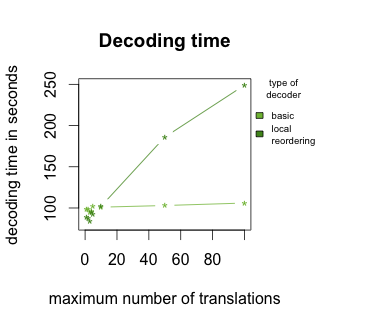
\includegraphics[width=\textwidth]{figures/k_time.png}
    \caption{TODO include correct image!}\label{decode3}
\end{figure}
